\section{Datastores}

\paragraph{Proxmox} supports all storage technologies available for Debian Linux, for example LVM for local storage or iSCSI for network attached storage.
\\
Here is the table for the currently supported storage types including if they are shared and support snapshots.

% chktex-file 44
\begin{table}[H]
    \label{tab:storageTable}
    \centering
    \caption{Proxmox available storage types}
    \begin{tabular}{|l|l|l|l|l|}
        \hline
        \textbf{Description} & \textbf{Level} & \textbf{Shared} & \textbf{Snapshots} & \textbf{Stable} \\ \hline
        ZFS (local)           & both           & no              & yes                & yes             \\ \hline
        Directory             & file           & no              & no                 & yes             \\ \hline
        BTRFS                 & file           & no              & yes                & technology preview \\ \hline
        NFS                   & file           & yes             & no                 & yes             \\ \hline
        CIFS                  & file           & yes             & no                 & yes             \\ \hline
        Proxmox Backup        & both           & yes             & n/a                & yes             \\ \hline
        GlusterFS             & file           & yes             & no                 & yes             \\ \hline
        CephFS                & file           & yes             & yes                & yes             \\ \hline
        LVM                   & block          & no              & no                 & yes             \\ \hline
        LVM-thin              & block          & no              & yes                & yes             \\ \hline
        iSCSI/kernel          & block          & yes             & no                 & yes             \\ \hline
        iSCSI/libiscsi        & block          & yes             & no                 & yes             \\ \hline
        Ceph/RBD              & block          & yes             & yes                & yes             \\ \hline
        ZFS over iSCSI        & block          & yes             & yes                & yes             \\ \hline
    \end{tabular}
\end{table}

\paragraph{vSphere} supports the following 4 datastores:

\begin{itemize}
    \item VMFS (Virtual Machine File System): A special file system optimized for storing virtual machines.
    \item NFS (Network File System): A file system that allows a client to access files over a network.
    \item vSAN (Virtual Storage Area Network): A storage area network that is integrated with vSphere.
    \item vVol (Virtual Volumes): A storage container in vCenter and vShpere Client.
\end{itemize}

vSAN tries to aggregate the local storage of all hosts in a cluster to create a shared storage pool. vVol uses an existing SAN/NAS an virtaulizes it into a storage container that is better usable by the ESXi hosts.

\begin{figure}[H]
    \centering
	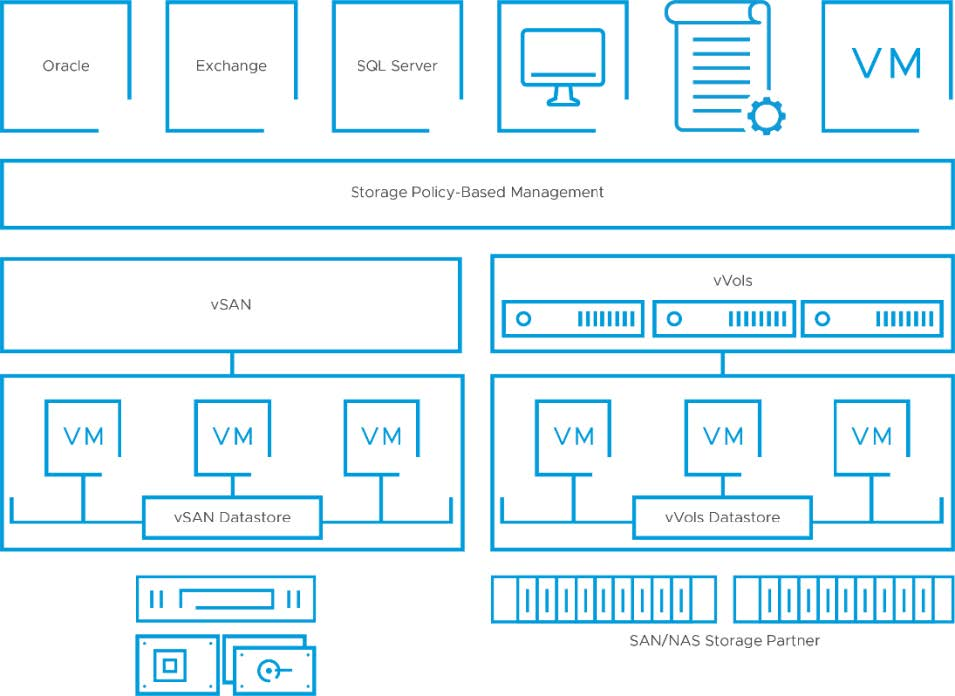
\includegraphics[width=0.8\linewidth]{vsan_vvol.jpg} % Figure image
	\caption{vSAN vs vVol} % Figure caption
	\label{fig:vSAN_vs_vVol} % Label for referencing with \ref{bear}
\end{figure}

Depending on the storage type vSphere supports different features.

\begin{table}[h!]
    \centering
    \caption{Storage Type Capabilities}
    \begin{tabular}{|l|l|l|l|l|l|}
    \hline
    \textbf{Storage Type} & \textbf{vMotion} & \textbf{Datastore} & \textbf{RDM} & \textbf{VM Cluster} & \textbf{VMware HA and DRS} \\ \hline
    Local Storage         & No               & VMFS                & No          & Yes                & No                          \\ \hline
    Fibre Channel         & Yes              & VMFS                & Yes         & Yes                & Yes                         \\ \hline
    iSCSI                 & Yes              & VMFS                & Yes         & Yes                & Yes                         \\ \hline
    NAS over NFS          & Yes              & NFS 3 and NFS 4.1   & No          & No                 & Yes                         \\ \hline
    \end{tabular}
\end{table}
